\documentclass[11pt]{amsart}
\usepackage{geometry}                % See geometry.pdf to learn the layout options. There are lots.
\geometry{letterpaper}                   % ... or a4paper or a5paper or ... 
%\geometry{landscape}                % Activate for for rotated page geometry
%\usepackage[parfill]{parskip}    % Activate to begin paragraphs with an empty line rather than an indent
\usepackage{graphicx}
\usepackage{amssymb}
\usepackage{amsmath}
\usepackage{epstopdf}
\usepackage[linesnumbered,vlined,algoruled]{algorithm2e}
\usepackage{url}
\usepackage{mathtools}
\DeclarePairedDelimiter{\ceil}{\lceil}{\rceil}
\DeclarePairedDelimiter{\floor}{\lfloor}{\rfloor}
\DeclareGraphicsRule{.tif}{png}{.png}{`convert #1 `dirname #1`/`basename #1 .tif`.png}
\DeclareMathOperator*{\argmax}{arg\,max}
\DeclareMathOperator{\argmin}{arg\,min}

\title{Computing Accurate Quantiles Using 1-D Clustering}
\author{Ted Dunning}
\email{ted.dunning@gmail.com}
\date{}                                           % Activate to display a given date or no date
\begin{document}
\begin{abstract}
An on-line algorithm for computing approximations of rank-based statistics is presented that allows controllable accuracy.  Moreover, this new algorithm can be used to compute hybrid statistics such as trimmed means in additional to computing arbitrary quantiles.  An unusual property of the method is that it allows a quantile $q$ to be computed with an accuracy relative to $q (1-q)$ rather than with an absolute accuracy as with most methods.  
\end{abstract}
\maketitle
\section{Introduction}
Given a sequence of numbers, it is often desirable to compute rank-based statistics such as the median, 95-th percentile or trimmed means in an on-line fashion, keeping only a small data structure in memory.  Traditionally, such statistics were often computed by sorting all of the data and then either finding the quantile of interest by interpolation or by processing all samples within particular quantiles.  This sorting approach is infeasible for very large datasets which has led to interest in on-line approximate algorithms.

One early algorithm for computing on-line quantiles is described in \cite{Chen2000}.  In that work specific quantiles were computed by incrementing or decrementing an estimate by a value proportional to the simultaneously estimated probability density at the desired quantile.  This method is plagued by a circularity in that estimating density is only possible by estimating yet more quantiles.  Moreover, this work did not allow the computation of hybrid quantities such as trimmed means.

An alternative approach is described in \cite{qdigest}.  In this work, incoming values are assumed to be integers of fixed size. Such integers can trivially be arranged in a perfectly balanced binary tree where the leaves correspond to the integers and the interior nodes correspond to bit-wise prefixes. This tree forms the basis of the data structure known as a Q-digest.  The idea behind a Q-digest is that in the uncompressed case, counts for various values are assigned to leaves of the tree.  To compress this tree, sub-trees are collapsed and counts from the leaves are aggregated into a single node representing the sub-tree such that the maximum count for any collapsed sub-tree is less than a threshold that is a small fraction of the total number of integers seen so far.  Any quantile can be computed by traversing the tree in left prefix order, adding up counts until the desired fraction of the total is reached.  At that point, count for the last sub-tree traversed can be used to interpolate to the desired quantile within a small and controllable error.  The error is bounded because the count for each collapsed sub-tree is bounded.

The two problems with the Q-digest are that it depends on the tree structure being known ahead of time and that the error bounds do not apply if the algorithm is used in an on-line fashion.  Adapting the Q-digest to use an balanced tree over arbitrary elements is difficult.  This difficulty arise because rebalancing the tree involves sub-tree rotations and these rotations may require reapportionment of previously collapsed counts in complex ways.  This reapportionment can have a complex affect on the accuracy of the algorithm and in any case make the implementation much more complex because the concerns of counting cannot be separated from the concerns of maintaining a balanced tree.  Another problem with Q-digests is that if they are subjected to compression during building, it isn't entirely clear how to handle compressed counts that move high above the leaves, but which eventually have non-trivial counts at a lower level in the tree.  The proof of correctness for Q-digests ignores this complication by only considering the case where counts are compressed after being collected on the leaves.  It would be desirable to have error bounds that apply to a completely on-line data structure.

The work described here shows how the fundamental idea of a Q-digest can be easily extended to values in $\mathbb R$ without the complexity of apportioning counts during tree rebalancing.  Indeed, this new data structure completely eliminates the concept of the tree itself, maintaining only the concept of collapsing groups of observations in a way that preserves accuracy.  This new algorithm, known as $1-d$ clustering, has well-defined and easily proven error bounds and allows parallel on-line operation.  A novel aspect of the variant of $1-d$ clustering described here is that accuracy for estimating the $q$ quantile is relative to $q(1-q)$.  This is in contrast to earlier algorithms which had errors independent of $q$.  The relative error bounds of $1-d$ cluster is convenient when computing quantiles for very small $q$ or for $q$ near $1$.  As with the Q-digest algorithm, the accuracy/size trade-off can be controlled by setting a single compression parameter.

\section{The Algorithm}
The algorithm for $1-d$ clustering is quite simple.  An initially empty ordered list of centroids, $C = [ c_1 \ldots c_m ]$ is kept.  Each centroid consists of a mean and a count.  To add a value $x_n$, the set of centroids is found that have minimum distance to $x_n$.  This set is reduced by retaining only centroids with a count less than $\delta q (1-q) n$.  If more than one centroid remains, one is selected at random.  If a centroid is found, then $x_n$ is added to that centroid and the next input is considered.  If no satisfactory centroid is found, then $x_n$ is used to form a new centroid and the next point is considered.  This procedure is given more formally in Algorithm \ref{alg:full}.
 \begin{algorithm}[tb]
\SetKw{KwTo}{in}\SetKwFor{For}{for}{\string:}{}
\SetKwIF{If}{ElseIf}{Else}{if}{:}{elif}{else:}{}
\SetKwFor{While}{while}{:}{fintq}
\SetKwFor{For}{for}{\string:}{}
 \label{alg:full}
\SetNoFillComment
\KwIn{Ordered set of weighted centroids $C = \lbrace \rbrace$, sequence of real-valued, weighted points $X = \lbrace (x_1, w_1),\ldots (x_N, w_N)\rbrace$, and accuracy tolerance $\delta$}
\KwOut{final set $C=[c_1 \ldots c_m]$ of weighted centroids} 
\For{$(x_n, w_n) \in X$} {
  $z = \min | c_i.\mathtt{mean} - x |$\;
  $S = \lbrace c_i  :  |c_i.\mathtt{mean} - x| = z \wedge c_i.\mathtt{count} + w_n \le 4n\delta q(c_i) (1-q(c_i)) \rbrace $ \;
   \uIf {$S \ne \lbrace \rbrace$} {
       Sample $c_j \sim \mathrm{Uniform}( S)$\;
       $c_j.\mathtt{count} \gets c_j.\mathtt{count} + 1$ \;
       $c_j.\mathtt{mean} \gets c_j.\mathtt{mean} + (x - c_j.\mathtt{mean})/c_j.\mathtt{count}$\;
     } 
     \Else {
        $C \gets C + [x, 1]$\;
      }
      \If {$|C| > K/\delta$} {
         $C \gets \mathtt{cluster}(\mathtt{permute}(C)) $ \;
       }
} 
\Return $ C $\\
\caption{$1-d$ Clustering}
\end{algorithm}

In this algorithm, a centroid object contains a mean and and a count.  Updating such an object with a new data-point $x$ is done using Welford's method \cite{wiki:welford, knuth2welford, welford62}.

The number of points assigned to each centroid is limited to roughly $\max(1, \floor{4N\delta q(1-q})$ where $q$ is the quantile for the approximate mean of the centroid.  The algorithm approximates $q$ by summing the weights for all of the centroids ordered before the centroid in question.  For centroids with identical means, order of creation is used as a tie-breaker.  In addition, half of the weight of the current centroid is included in the sum.  In order to compute this sum quickly, the centroids are stored in a balanced binary tree that keeps sums of each sub-tree.  Figure \ref{fig:gamma-sizes} shows actual centroid weights from 5 runs with a $\Gamma(0.1, 0.1)$ distribution plotted against the ideal bound.

The use of a bound on centroid size that becomes small for extreme values of $q$ is useful because it allows bounds error, but may also be problematic in some cases.  If the values of $X$ are sufficiently ordered, then $C$ will grow unreasonably because new extreme values of $X$ will always be assigned to new centroids.  To avoid this pathology, if the number of centroids becomes excessive, the set of centroids is collapsed by recursively applying $1-d$ clustering to the centroids themselves in randomized order.  This method of recursive clustering can also be used to parallelize $1-d$ by independently processing sub-sequences of $X$ and then combining the results by clustering the concatenation of all centroids.

Initial versions of this algorithm tried to use the centroid index $i$ as a surrogate for $q$, applying a correction to account for the fact that extreme centroids have less weight.  Unfortunately, it was difficult to account for the fact that the distribution of centroid weights changes during the course of running the algorithm.  Initially all weights are $1$.  Later, some weights become substantially larger.  This means that the relationship between $i$ and $q$ changes from completely linear to highly non-linear in a stochastic way.  This made it difficult to avoid too large or too small cutoff for centroids resulting in either too many centroids or poor accuracy.
\begin{figure}[htb] %  figure placement: here, top, bottom, or page
   \centering
   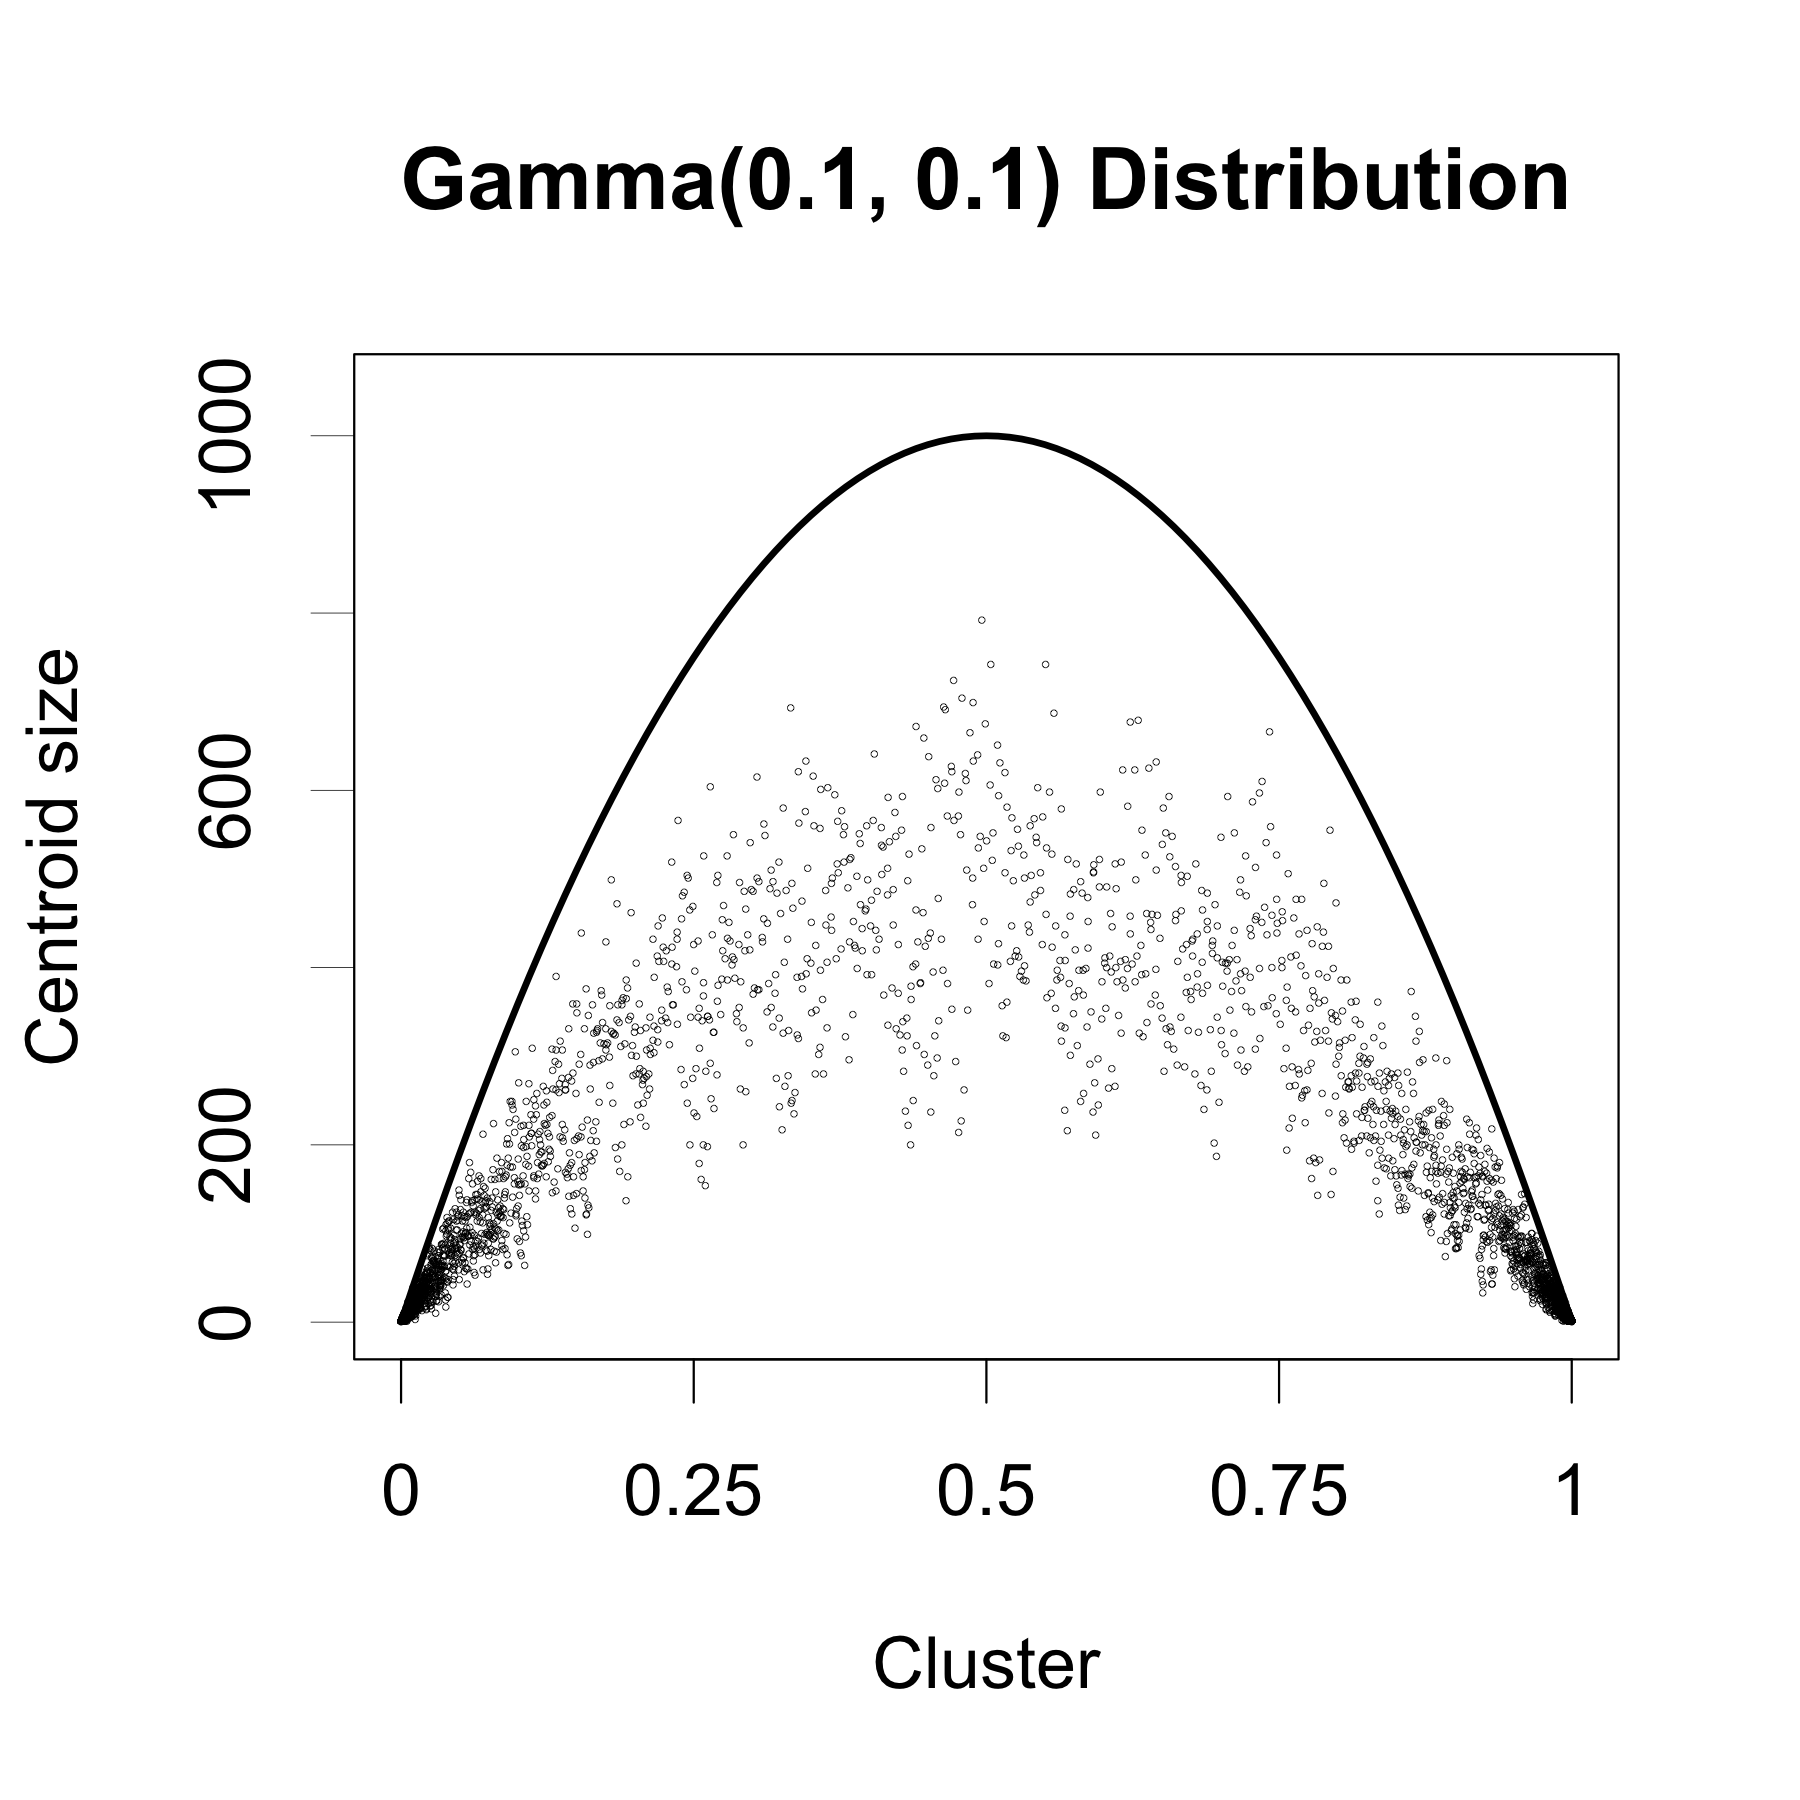
\includegraphics[width=3in]{gamma-sizes.png} 
   \caption{The accuracy of the size limit approximation used in the $1-d$ clustering algorithm.  The solid line indicates the intended size limit.  In addition, this diagram also shows actual centroid weights for 5 test runs on $100,000$ samples from a $\Gamma(0.1, 0.1)$ distribution.  In spite of the underlying distribution being skewed by roughly $30$ orders of magnitude of difference in probability density, the centroid weight distribution is bounded and symmetric 
 as intended.}
   \label{fig:gamma-sizes}
\end{figure}

The key property of this algorithm is that the final list of centroids $C$ is very close to what would have been obtained by simply sorting and then grouping adjacent values in $X$ into groups with the desired size bounds.  Clearly, such groups could be used to compute all of the rank statistics of interest here and if there are bounds on the sizes of the groups, then we have comparable bounds on the accuracy of the rank statistics in question.

That this algorithm does produce such an approximation is more difficult to prove rigorously, but an empirical examination is enlightening.  Figure \ref{fig:deviation} shows the deviation of samples assigned to centroids uniform and highly skewed distributions.  These deviations are normalized by the half the distance between the adjacent two centroids.
\begin{figure}[htb] %  figure placement: here, top, bottom, or page
   \centering
   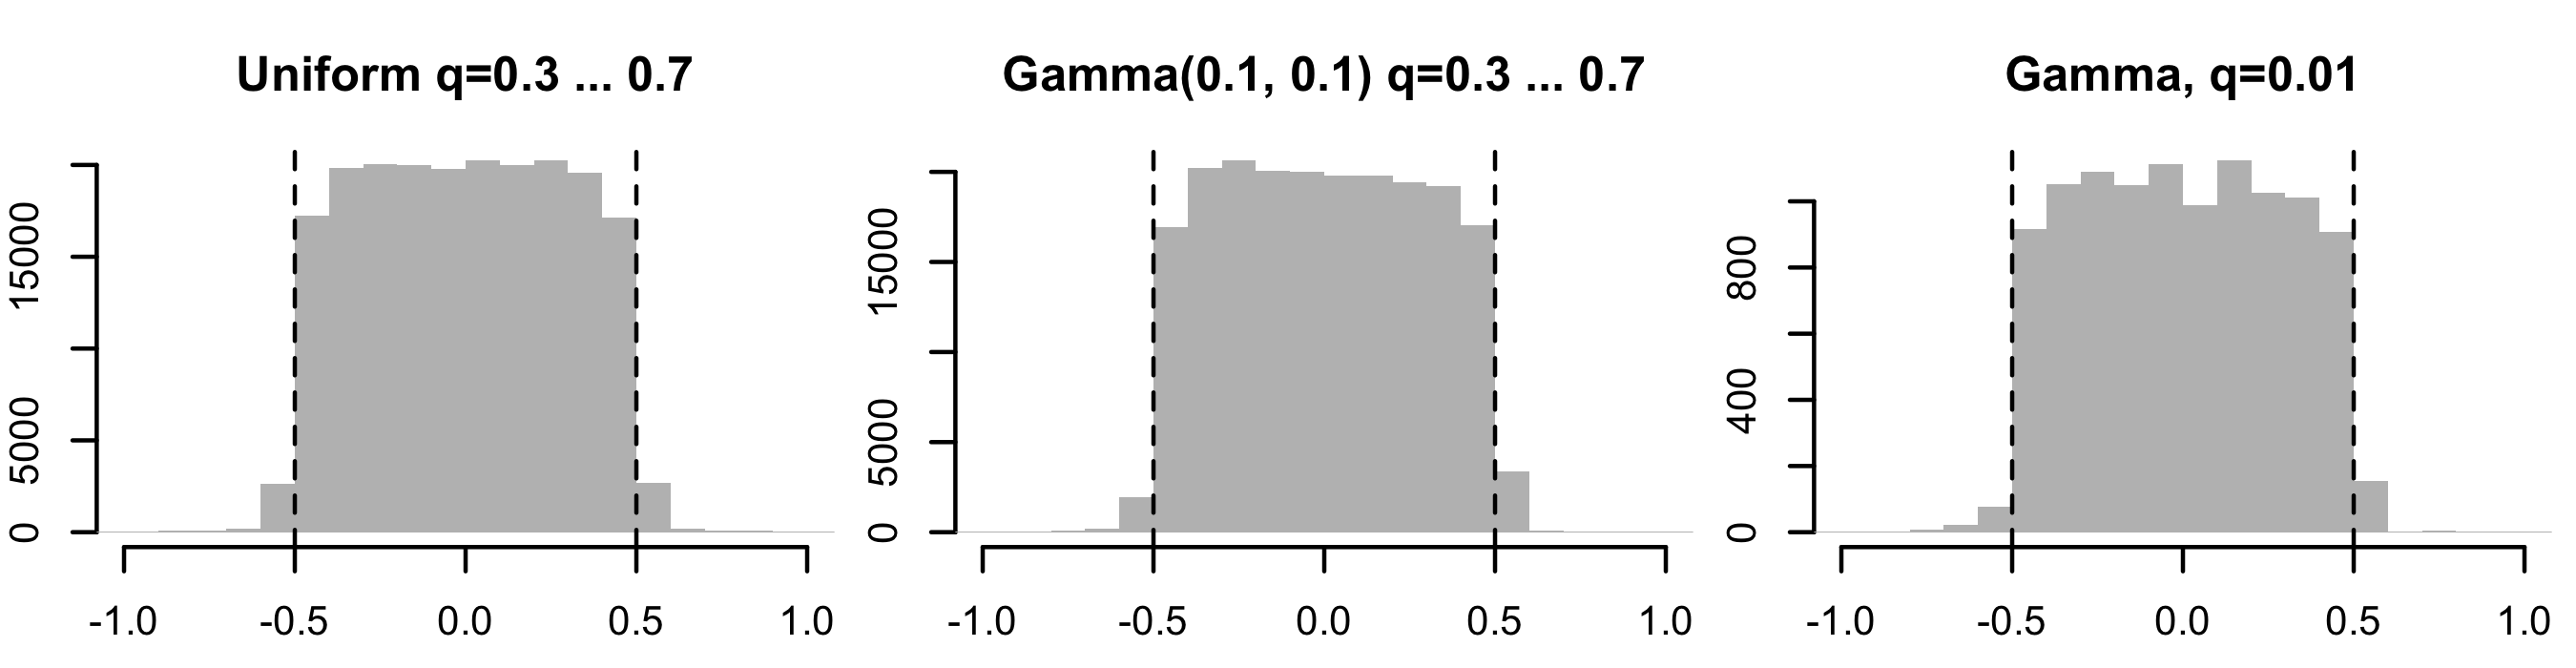
\includegraphics[width=4.5in]{deviation.png} 
   \caption{The deviation of samples assigned to a single centroid.  The horizontal axis is scaled to the distance to the adjacent centroid so a value of 0.5 is half-way between the two centroids. There are two significant observations to be had here.  The first is that relatively few points are assigned to a centroid that are beyond the midpoint to the next cluster.  This bears on the accuracy of this algorithm.  The second observation is that samples are distributed relatively uniformly between the boundaries of the cell.  This affects the interpolation method to be chosen when working with quantiles. The three graphs show, respectively, centroids from $q \in [0.3, 0.7]$ from a uniform distribution, centroids from the same range of a highly skewed $\Gamma(0.1, 0.1)$ and centroids from $q \in [0.01, 0.015]$ in a $\Gamma(0.1, 0.1)$ distribution.  This last range is in a region where skew on the order of $10^{22}$ is found. }
   \label{fig:deviation}
\end{figure}
This relatively uniform distribution for deviations among the samples assigned to a centroid is found for uniformly distributed samples as well as for extremely skewed data.  For instance, the $\Gamma(0.1, 0.1)$ distribution has a $0.01$ quantile of $6.07 \times 10^{-20}$, a median of $0.006$ and mean of the distribution is $1$.  This means that the distribution is very skewed.  In spite of this, samples assigned to centroids near the first percentile are not noticeably skewed within the centroid.  The impact of this uniform distribution is that linear interpolation allows accuracy considerably better than $1/\delta$ even for quantiles near $q=0.5$.

\subsection{Finding the cumulative distribution at a point}
Algorithm \ref{alg:quantile} shows how to compute the cumulative distribution $P(x)=\int_{-\infty}^x p(\alpha) \, d\alpha$ by summing the contribution of uniform distributions centered at each the centroids.  Each of the centroids is assumed to extend symmetrically around the mean for half the distance to the next centroid mean.

 \begin{algorithm}[b]
 \label{alg:quantile}
\SetKw{KwTo}{in}\SetKwFor{For}{for}{\string:}{}
\SetKwIF{If}{ElseIf}{Else}{if}{:}{elif}{else:}{}
\SetKwFor{While}{while}{:}{fintq}
\SetKwFor{For}{for}{\string:}{}
\SetNoFillComment
\KwIn{Centroids derived from distribution $p(x)$, $C = [ \ldots [m_i, s_i, k_i] \ldots ]$ , value $x$ }
\KwOut{Estimated value of $q = \int_{-\infty}^x p(\alpha) d \alpha$} 
$t = 0$, $N = \sum_i k_i$\;
\For {$i \in 1\ldots m$} {
    \uIf {$i < m$} {
      $\Delta \gets (c_{i+1}.\mathtt{mean} - c_i.\mathtt{mean})/2$\;
    } \Else {
      $\Delta \gets (c_{i}.\mathtt{mean} - c_{i-1}.\mathtt{mean})/2$\;
    }
    $z = \max(-1, (x-m_i)/\Delta)$\;
  \If {$z < 1$} {
    \Return $(t + \frac{k_i} N \frac{z+1} {2})$
  }
  $t \gets t + k_i$\;
}
\Return $1$
\caption{Estimate quantile $C.\mathtt{quantile}(x)$}
\end{algorithm}

For all centroids except one, this contribution will be either $0$ or $k_i/N$ and the one centroid which straddles the desired value of $x$ will have a contribution somewhere between $0$ and $k_i/N$. Moreover, since each centroid has count at most $\delta N/4$ the accuracy of $q$ should be accurate on a scale of $\delta/4$.  Typically, the accuracy will be even better due to the interpolation scheme used in the algorithm and because the largest centroids are only for values of $q$ near $0.5$.

The empirical justification for using a uniform distribution for each centroid can be seen by referring to again to Figure \ref{fig:deviation}.  
\subsection{Inverting the cumulative distribution}
Computing an approximation of the $q$ quantile of the data points seen so far can be done by ordering the centroids by ascending mean.  The running sum of the centroid counts will range from $0$ to $N=\sum k_i$.  One particular centroid will have a count that straddles the desired quantile $q$ and interpolation can be used to estimate a value of $x$.  This is shown in Algorithm \ref{alg:estimate-quantile}.   Note that at the extreme ends of the distribution as observed, each centroid will represent a single sample so maximum resolution in $q$ will be retained.

 \begin{algorithm}[b]
 \label{alg:estimate-quantile}
\SetKw{KwTo}{in}\SetKwFor{For}{for}{\string:}{}
\SetKwIF{If}{ElseIf}{Else}{if}{:}{elif}{else:}{}
\SetKwFor{While}{while}{:}{fintq}
\SetKwFor{For}{for}{\string:}{}
\SetNoFillComment
\KwIn{Centroids derived from distribution $p(x)$, $C = [c_1 \ldots c_m ]$ , value $q$}
\KwOut{Estimated value $x$ such that $q = \int_{-\infty}^x p(\alpha) d \alpha$} 
$t = 0$, $q \gets q \sum c_i.\mathtt{count}$\;
\For {$i \in 1\ldots m$} {
  $k_i = c_i.\mathtt{count}$\;
  \uIf {$q < k_i$} {
    \uIf {$i > 1$} {
      $\Delta \gets (c_{i+1}.\mathtt{mean} - c_{i-1}.\mathtt{mean})/2$\;
    } \uElseIf {$i < m$} {
      $\Delta \gets (c_{i+1}.\mathtt{mean} - c_i.\mathtt{mean})$\;
    } \Else {
      $\Delta \gets (c_{i}.\mathtt{mean} - c_{i-1}.\mathtt{mean})$\;
    }
    \Return $m_i + \left( \frac {q-t} {k_i} - \frac 1 2 \right) \Delta$
  } 
  $t \gets t + k_i$
}
\Return $ c_m.\mathtt{mean}$
\caption{Estimate value at given quantile $C.\mathtt{icdf}(q)$}
\end{algorithm}

\subsection{Computing the trimmed mean}
The trimmed mean of $X$ for the quantile range $Q = [q_0,q_1]$ can be computed by computing a weighted average of the means of centroids that have quantiles in $Q$.  For centroids at the edge of $Q$, a pro-rata weight can be used that is based on an interpolated estimate of the fraction of the centroid's samples that are in $Q$.  This method is shown as Algorithm \ref {alg:estimate-trimmed-mean}.

 \begin{algorithm}[b]
 \label{alg:estimate-trimmed-mean}
\SetKw{KwTo}{in}\SetKwFor{For}{for}{\string:}{}
\SetKwIF{If}{ElseIf}{Else}{if}{:}{elif}{else:}{}
\SetKwFor{While}{while}{:}{fintq}
\SetKwFor{For}{for}{\string:}{}
\SetNoFillComment
\KwIn{Centroids derived from distribution $p(x)$, $C = [ \ldots [m_i, s_i, k_i] \ldots ]$ , limit values $q_0, q_2$}
\KwOut{Estimate of mean of values $x \in [q_0, q_1]$} 
$s = 0$, $k = 0$\;
$t = 0$, $q_1 \gets q_1 \sum k_i$, $q_1 \gets q_1 \sum k_i$\;
\For {$i \in 1\ldots m$} {
  $k_i = c_i.\mathtt{count}$\;
  \uIf {$q_1 < t+k_i$} {
    \uIf {$i > 1$} {
      $\Delta \gets (c_{i+1}.\mathtt{mean} - c_{i-1}.\mathtt{mean})/2$\;
    } \uElseIf {$i < m$} {
      $\Delta \gets (c_{i+1}.\mathtt{mean} - c_i.\mathtt{mean})$\;
    } \Else {
      $\Delta \gets (c_{i}.\mathtt{mean} - c_{i-1}.\mathtt{mean})$\;
    }
    $\eta = \left( \frac {q-t} {k_i} - \frac 1 2 \right) \Delta$\;
    $s \gets s + \eta \,k_i \,c_i.\mathtt{mean}$\;
    $k \gets k + \eta \,k_i$\;
  } 
  \uIf {$q_2 < t+k_i$} {
    \uIf {$i > 1$} {
      $\Delta \gets (c_{i+1}.\mathtt{mean} - c_{i-1}.\mathtt{mean})/2$\;
    } \uElseIf {$i < m$} {
      $\Delta \gets (c_{i+1}.\mathtt{mean} - c_i.\mathtt{mean})$\;
    } \Else {
      $\Delta \gets (c_{i}.\mathtt{mean} - c_{i-1}.\mathtt{mean})$\;
    }
    $\eta = \left(\frac 1 2 - \frac {q-t} { k_i}  \right) \Delta$\;
    $s \gets s - \eta \,k_i \,c_i.\mathtt{mean}$\;
    $k \gets k - \eta \,k_i$\;
  } 
  $t \gets t + k_i$
}
\Return $s/k$
\caption{Estimate trimmed mean.  Note how centroids at the boundary are included on a {\em pro rata} basis.}
\end{algorithm}
\section{Empirical Assessment}
\subsection{Accuracy of estimation for uniform and skewed distributions}
Figure \ref{fig:uniform-error} shows the error levels achieved with $1-d$ clustering in estimating quantiles of 100,000 samples from a uniform and from a skewed distribution.  In these experiments $\delta=0.01$ was used since it provides a good compromise between accuracy and space.  There is no visible difference in accuracy between the two underlying distributions in spite of the fact that the underlying densities differ by more roughly 30 orders of magnitude.  The accuracy shown here is computed by comparing the computed quantiles to the actual empirical quantiles for the sample used for testing and is shown in terms of $q$ rather than the underlying sample value.  At extreme values of $q$, the actual samples are preserved as centroids with weight $1$ so the observed for these extreme values is zero relative to the original data.  For the data shown here, at $q=0.001$, the maximum weight on a centroid is just above $4$ and centroids in this range have all possible weights from $1$ to $4$.  Accuracy is, not surprising, just a few parts per million or less.

Obviously, relatively small numbers of samples such as are used in these experiments, the accuracy of $1-d$ clustering as an estimate of the quantiles of the underlying distribution cannot be better than the accuracy of these estimates computed using the entire sample.  For the experiments here, the errors due to sampling completely dominate the errors introduced by $1-d$ sampling, especially at extreme values of $q$.

It should be noted that using a Q-digest implemented with longs is only able to store data with about 20 significant decimal figures.  This means that such a Q-digest would be inherently unable to even estimate the quantiles of the $\Gamma$ distribution tested here.
\subsection{Storing $1-d$ clusterings}
For the accuracy setting and test data used in these experiments, the $1-d$ clustering produced $840-850$ centroids.  The results of $1-d$ clustering can thus be stored by storing this many centroid means and weights.  If centroids are kept as double precision floating point numbers and counts kept as integers, the $1-d$ clusterings resulting from from the accuracy tests described here would require just over 10 kilobytes of storage for any of the distributions tested.

This size can be substantially decreased, however.  One simple option is to store differences between centroid means and to use a variable byte encoding such as zig-zag encoding to store the cluster size.  The differences between successive means are at least three orders of magnitude smaller than the means themselves so using single precision floating point to store these differences can allow the $1-d$ clusterings from the tests described here to be stored in about $4.5$ kilobytes while still regaining nearly 10 significant figures of accuracy in the means.  This is roughly equivalent to the precision possible with a Q-digest operating on 32 bit integers, but the dynamic range of $1-d$ clustering will be considerably higher and the accuracy is considerably better.

\subsection{Space/Accuracy Trade-off}
\subsection{Speed}

\begin{figure}[htb] %  figure placement: here, top, bottom, or page
   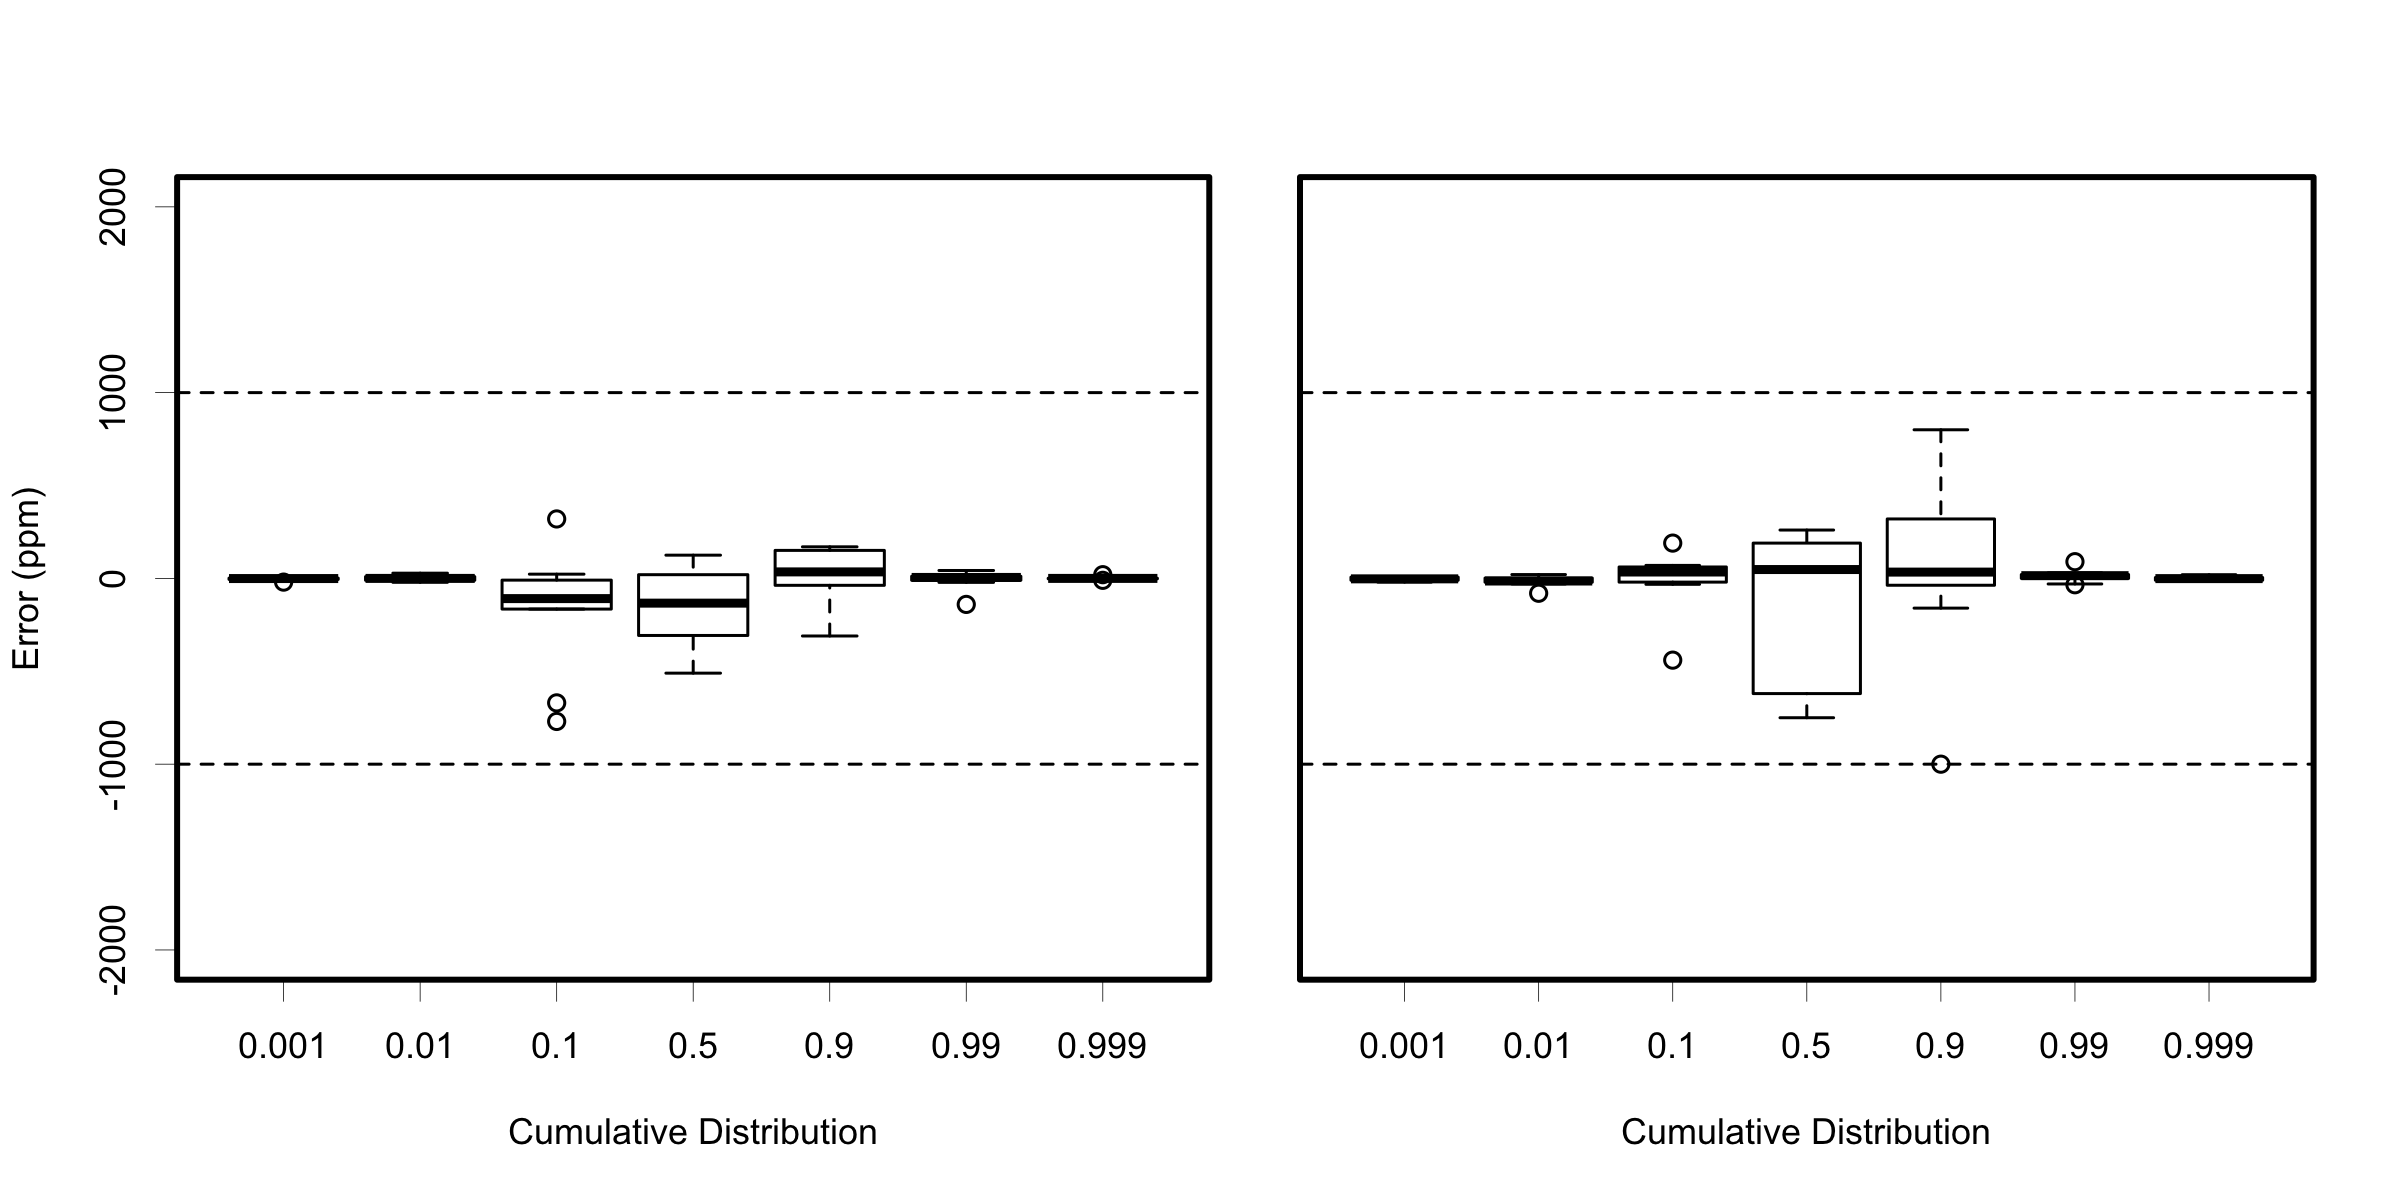
\includegraphics[width=6in]{error.png} 
   \caption{The absolute error of the estimate of the cumulative distribution function $q = \int_{-\infty}^x p(\alpha) \, d\alpha$ for the uniform distribution for 5 runs, each with 100,000 data points.  As can be seen, the error is dramatically decreased for very high or very low quantiles (to a few parts per million).  The precision setting used here, $\delta = 0.01$, would result in uniform error of 10,000 ppm without adaptive bin sizing and interpolation.}
   \label{fig:uniform-error}
\end{figure}

%\subsection{}
\bibliographystyle{alpha}
\bibliography{refs}{}

\end{document}  